\section{Every copy, its count, and an exact transversal}
\label{sec:copies}

The proofs of this section are valid for an anchor size \(s\) whenever
the full-pattern pinning conclusion holds. We will use \(s=3\) for the
main construction. Keeping \(s\) visible in the sampling formulas will
also identify exactly where anchor size matters.

\begin{theorem}[Complete classification of copies]
\label{thm:classification}
Every copy of \(H\) in \(A_h\) uses mode \(W_{h,p\bmod2}^-\) for a
unique leaf \(p\). Its body rows are that leaf row and an arbitrary
dummy row. Its body columns are that leaf column and either of the two
columns in \(C_{h-1}^-(\pi(p))\). Conversely, all these choices, together
with arbitrary representatives of the \(2s\) anchor groups of the mode,
give a copy.
\end{theorem}
\begin{proof}
Pinning fixes the mode and all four body roles. It remains to impose
the orders \eqref{eq:orders}, entries \eqref{eq:entries}, and the body
\(P=\left(\begin{smallmatrix}1&0\\1&1\end{smallmatrix}\right)\).

In a \(V_i^+\) body, let \(p\) index the child row, \(a\) the parent
row, and \(b\) the parent column. The row order requires \(\pi(p)\le a\).
The bottom-right one requires \(a\le b\). Hence \(\pi(p)\le b\), so
the top-right entry is one, a contradiction.

In a \(V_i^-\) body, the row order requires \(\pi(p)\ge a\), and
the top-right zero requires \(a\ge b\). Thus \(\pi(p)\ge b\), making
the bottom-right entry zero. This is also impossible.

In a \(W_{i,d}^+\) body, let \(p,q\) be the child row and column
indices and \(b\) the parent column index. Column order gives
\(b\le\pi(q)\), while the top-left one gives \(\pi(p)\le b\).
The two child indices have the same parity, so \(p\le q\). The
top-right entry is then one, contradicting its prescribed zero.

For \(W_{i,d}^-\), column order and the top-right zero give
\[
 \pi(q)\le b\le\pi(p).
\]
Equal parity implies \(p\ge q\). If \(i<h\), the top-left entry
\(\one[p<q]\) is zero, so no copy exists. At \(i=h\) the shared
leaf entry is \(\one[p\le q]\); it equals one only when \(p=q\).
The displayed inequalities then force \(b=\pi(p)\).

These necessary conditions are sufficient. The leaf column precedes
its parent's minus column, the leaf row precedes the dummy row, and
the body entries are exactly \(1,0,1,1\). The anchor signatures and
anchor order are already correct. This proves both directions.
\end{proof}

\begin{corollary}[Exact count]
\label{cor:exact-count}
For anchor size \(s\),
\begin{equation}
 N_H(A_h)=2m^{2s+2}.
 \label{eq:exact-general-count}
\end{equation}
\end{corollary}
\begin{proof}
There are \(m\) possible leaves, two parent-column positions for each
leaf, \(m\) dummy rows, and \(m\) choices in each of the \(2s\) anchor
groups. Their product is \(2m^{2s+2}\). Different choices give distinct
increasing row and column maps, and the classification proves completeness.
\end{proof}

Let \(\mathcal L_h=\bigcup_{0\le p<m}R_h(p)\times C_h(p)\) be the
\(m\)-cell leaf diagonal. In each copy it is the body entry \((1,1)\),
that is, pattern position \((s+1,s+1)\), that lies on \(\mathcal L_h\).

\begin{theorem}[Exact packing and covering of existing copies]
\label{thm:packing}
Let \(\tau_H(A_h)\) be the minimum number of cells meeting every existing
\(H\)-copy and \(\nu_H(A_h)\) the maximum number of entry-disjoint copies.
Then
\begin{equation}
 \tau_H(A_h)=\nu_H(A_h)=m.
 \label{eq:packing}
\end{equation}
Indeed, \(m\) copies can be chosen with mutually disjoint row sets and
mutually disjoint column sets.
\end{theorem}
\begin{proof}
The diagonal \(\mathcal L_h\) meets every copy, so \(\tau_H(A_h)\le m\).
For each leaf \(p\), choose its dummy row using a different representative
of \(R_*\). Assign the two columns of each parent-minus block bijectively
to that parent's two children. In every anchor group of the relevant
parity mode choose the representative indexed by \(p\), using a fixed
indexing of each size-\(m\) group. Different leaves in the same mode use
different representatives; different modes have disjoint groups.

The resulting \(m\) copies have disjoint selected rows and disjoint
selected columns. Hence they are entry-disjoint and any transversal
needs at least one different cell for each. The inequalities
\(m\le\nu_H(A_h)\le\tau_H(A_h)\le m\) prove the claim.
\end{proof}

Changing the leaf diagonal itself is not a successful repair. If its
ones are changed to zeros, a leaf \(p\), a dummy row, a column of
\(C_{h-1}^+(\pi(p))\), and the leaf column now form \(P\) in mode
\(W_{h,p\bmod2}^+\). Their anchor signatures are unchanged. Thus
destroying all original copies can create a new complete family of copies.

\section{Exact distance under arbitrary entry changes}
\label{sec:distance}

\begin{theorem}[Exact repair]
\label{thm:repair}
Every \(H\)-free matrix differs from \(A_h\) in at least \(m^2\) cells.
The matrix \(A_h^{\mathrm{rep}}\) of \eqref{eq:repair} is \(H\)-free.
Consequently the minimum number of entry changes is exactly \(m^2\).
\end{theorem}
\begin{proof}
The lower bound is the cellwise propagation argument of~\cite{OAI190},
which we include with the dependence and sampling details explicit.
Let \(B\) differ from \(A_h\) on a set \(E\) of fewer than \(m^2\)
cells. Partition each axis into its anchor groups, dummy group, signed
variable classes below the leaves, and one shared leaf class. Every
class in this partition has size \(m\).

Choose a leaf \(z\) uniformly from \(\{0,\ldots,m-1\}\), and let
\(a_i=\lfloor z/2^{h-i}\rfloor\) be its ancestor at depth \(i\).
Conditional on \(z\), choose independently uniform representatives
\[
 x_i^\sigma\in R_i^\sigma(a_i),\qquad
 y_i^\sigma\in C_i^\sigma(a_i),
\]
using the same representative for the two names at the leaves. Also
choose independently a representative from every anchor group and
each dummy group, denoting the latter by \(x_*,y_*\).

Each variable representative is uniform on its full size-\(m\) class:
its node is chosen with probability \(2^{-i}\), and the conditional
block size is \(m/2^i\). Anchor and dummy choices are independent of
every choice on the opposite axis. The root row and column choices
are independent uniform choices in their fixed blocks. Hence any fixed
cell with at least one anchor or dummy coordinate, or with both
coordinates at the root level, is selected with probability \(m^{-2}\).
There is just one representative in every partition class, including
the shared leaf class. A union bound over changed cells of these types
therefore gives
\begin{equation}
 \Prob(\text{some selected protected cell lies in }E)
 \le |E|/m^2<1.
 \label{eq:protected}
\end{equation}
Fix a choice for which all these selected cells retain their original
values. No restriction is imposed on the other edited cells.

For each mode, its chosen anchors are intact, with the original
signatures to the chosen body positions. If \(B\) were \(H\)-free,
none of these chosen, correctly ordered bodies could equal \(P\).
The root values are
\[
 B(x_0^+,y_0^+)=1,\qquad B(x_0^-,y_0^-)=0.
\]
Suppose these values have reached depth \(i-1\). The \(V_i^+\) and
\(V_i^-\) bodies are respectively
\[
 \begin{pmatrix}1&B(x_i^+,y_{i-1}^+)\\1&1\end{pmatrix},
 \qquad
 \begin{pmatrix}1&0\\1&B(x_i^-,y_{i-1}^-)\end{pmatrix}.
\]
Their left columns are intact dummy incidences. Avoidance of \(P\)
forces the two unknown entries to be one and zero. With
\(d_i=a_i\bmod2\), the \(W_{i,d_i}^+\) and \(W_{i,d_i}^-\) bodies
are then
\[
 \begin{pmatrix}1&B(x_i^+,y_i^+)\\1&1\end{pmatrix},
 \qquad
 \begin{pmatrix}B(x_i^-,y_i^-)&0\\1&1\end{pmatrix}.
\]
Avoidance forces
\(B(x_i^+,y_i^+)=1\) and \(B(x_i^-,y_i^-)=0\).
All four bodies have the required parent-child orders by construction.
Induction reaches the shared leaf cell and assigns it both values.
This contradiction proves the lower bound. In particular the argument
allows arbitrary zero-to-one as well as one-to-zero changes.

For the upper bound, the structural proof in \cref{sec:structure}
establishes full-pattern pinning in \(A_h^{\mathrm{rep}}\).
The \(V\) modes have unchanged bodies and still contain no \(P\).
The \(W\) modes below depth \(h\) are also unchanged. At depth \(h\),
a \(W^+\) body has its required bottom-right entry in
\(R_*\times C_h\), and a \(W^-\) body has its required bottom-left
entry there. Both entries are now zero, so neither body can be \(P\).
All pinned modes are excluded. This proves freeness after exactly
\(m^2\) changes.
\end{proof}

\subsection{Consequences for removal functions}

For the main five-by-five pattern, the exact formulas are
\begin{equation}
 d=20h+2,\qquad \eps_h=d^{-2},\qquad
 \delta_h=2d^{-10}4^{-h}=2\eps_h^5 4^{-h}.
 \label{eq:five-density}
\end{equation}
If \(a=\log2/20\), this can also be written
\begin{equation}
 \delta_h=2e^{4a}\eps_h^5
        \exp\bigl(-2a\eps_h^{-1/2}\bigr).
 \label{eq:explicit-stretched}
\end{equation}
This is an exact identity on the construction sequence, not merely
an upper estimate. It immediately excludes every positive power-law
lower bound in \eqref{eq:polynomial-question}.

An all-small-\(\eps\) statement follows without hiding the rounding.
Define the optimal removal modulus
\[
 \mathcal R_H(\eps)=\inf\left\{
  \frac{N_H(A)}{n^{10}}: n\ge1,\ \dist_H(A)\ge\eps\right\}.
\]
For \(0<\eps\le22^{-2}\), put
\(h=\lfloor(\eps^{-1/2}-2)/20\rfloor\). Then \(h\ge1\),
\(\eps_h\ge\eps\), and
\begin{equation}
 \mathcal R_H(\eps)
 \le \frac{2}{(20h+2)^{10}4^h}.
 \label{eq:all-epsilon}
\end{equation}
In particular, for an absolute constant \(K\) and all sufficiently
small \(\eps\),
\[
 \mathcal R_H(\eps)
 \le K\eps^5\exp\bigl(-2a\eps^{-1/2}\bigr).
\]
Indeed \(d\le\eps^{-1/2}<d+20\), so \(d\ge\eps^{-1/2}/2\) once
\(\eps^{-1/2}\ge40\); the bounded rounding changes the exponential
factor by at most \(e^{40a}\).

\section{Exact finite sampling formulas}
\label{sec:finite-sampling}

Let \(R,C\) be independent uniform \(q\)-element subsets of the two
axes of \(A_h\), and let \(D\) mean that \(A_h[R,C]\) contains \(H\).
Write \(p=q/n\) and
\[
 \rho_j=\frac{\fall qj}{\fall nj}\quad(0\le j\le q),
 \qquad \rho_j=0\quad(j>q),
 \qquad \rho_0=1.
\]
For a leaf \(\ell\), let \(I_\ell\) indicate that its leaf row, its
matching leaf column, and at least one column in its two-element
parent-minus block have all been sampled. Define
\begin{equation}
 X=\sum_{\ell=0}^{m-1}I_\ell.
 \label{eq:X}
\end{equation}
This count records successful leaves, rather than the number of choices
of a parent column or the much larger number of completed copies.

\begin{proposition}[Coverage and the exact first moment]
\label{prop:coverage}
For every \(0\le q\le n\),
\begin{align}
 0\le\Prob(X>0)-\Prob(D)&\le(4s+1)e^{-q/d},
 \label{eq:coverage}\\
 \lambda_q:=\E X&=m\rho_1(2\rho_2-\rho_3),
 \label{eq:first-moment}\\
 \Prob(D)&\le\min\{1,\lambda_q\}\le\min\{1,2mp^3\}.
 \label{eq:sample-upper}
\end{align}
For the main pattern \(s=3\), the coverage coefficient is \(13\).
\end{proposition}
\begin{proof}
Detection requires a leaf witness by \cref{thm:classification}.
Conversely, a witness completes to a copy if the sample meets the dummy
row block and every anchor group of both final minus parity modes.
This sufficient coverage event concerns \(4s+1\) groups of size \(m\).
For any one such group its miss probability is
\[
 \frac{\binom{n-m}{q}}{\binom nq}
 \le(1-m/n)^q\le e^{-q/d},
\]
with a zero numerator when \(q>n-m\). A union bound proves
\eqref{eq:coverage}; no independence of the coverage events is needed.
For a fixed leaf, its row is sampled with probability \(\rho_1\).
Inclusion-exclusion for the matching column and either parent column
gives \(2\rho_2-\rho_3\). Independence of the two axes and summation
give \eqref{eq:first-moment}. Finally \(\rho_2\le p^2\) and the
union bound prove \eqref{eq:sample-upper}.
\end{proof}

\begin{proposition}[Factorial moments without replacement]
\label{prop:factorial}
For every positive integer \(r\),
\begin{align}
 \E\fall Xr={}&\rho_r
 \sum_{j=\lceil r/2\rceil}^{r}
 r!\binom{m/2}{j}\binom j{r-j}2^{2j-r}
 \sum_{a=0}^{j}(-1)^a\binom ja2^{j-a}\rho_{r+j+a}.
 \label{eq:factorial-moments}
\end{align}
Binomial coefficients outside their usual ranges are zero.
\end{proposition}
\begin{proof}
Expand \(\fall Xr\) over ordered tuples of \(r\) distinct leaves.
If they have \(j\) parents, exactly \(r-j\) parents contribute both
children and \(2j-r\) contribute one child. The number of tuples is
\[
 r!\binom{m/2}{j}\binom j{r-j}2^{2j-r}.
\]
Their \(r\) leaf rows are present with probability \(\rho_r\).
Their leaf columns must be present, and each of the \(j\) disjoint
parent pairs must be hit. Expand the latter event as the product of
\(\one_u+\one_v-\one_u\one_v\) for those pairs. Selecting both
parent columns in \(a\) pairs, rather than one in each, gives the
inner sum. This proves the exact identity.
\end{proof}

For example,
\begin{equation}
 \E\fall X2=\rho_2\left[
 m(2\rho_3-\rho_4)+m(m-2)(4\rho_4-4\rho_5+\rho_6)\right].
 \label{eq:second-moment}
\end{equation}
Therefore, when \(\lambda_q>0\), a completely explicit finite lower
bound is
\begin{equation}
 \Prob(D)\ge
 \max\left\{0,
 \frac{\lambda_q^2}{\lambda_q+\E\fall X2}
       -(4s+1)e^{-q/d}\right\}.
 \label{eq:sample-lower}
\end{equation}
This follows from Cauchy--Schwarz applied to
\(X\one_{X>0}\), followed by \eqref{eq:coverage}.

\subsection{Independent retention of positions}

Under Bernoulli sampling, retain each row with probability \(u\) and
each column with probability \(v\), independently. Put
\[
 U=1-(1-u)^m,\quad V=1-(1-v)^m,\quad
 A=U^sV^s,\quad t=2v-v^2.
\]
The probability that one final parity mode has all its anchor groups
available is \(A\). The dummy row block is hit with probability \(U\).

\begin{proposition}[Exact Bernoulli law]
\label{prop:bernoulli}
The witness probability generating function is
\begin{equation}
 \E z^X=\left[1-t+t(1-uv+uvz)^2\right]^{m/2}.
 \label{eq:pgf}
\end{equation}
The actual detection probability, including anchor and dummy coverage, is
\begin{align}
 G_{m,s}(u,v)=U\biggl\{&2A(1-A)
    \left[1-(1-tuv)^{m/2}\right]\notag\\
 &+A^2\left[1-\left(1-t(2uv-u^2v^2)\right)^{m/2}\right]\biggr\}.
 \label{eq:bernoulli-exact}
\end{align}
\end{proposition}
\begin{proof}
Each parent has two candidate leaf pairs and two parent columns. The
parent columns are hit with probability \(t\). Conditional on that
event, its two leaf row-column pairs are independently present with
probability \(uv\). Different parents use disjoint positions. This gives
\eqref{eq:pgf}.

The two parity-mode coverage events are independent of each other, the
body positions, and the dummy rows. If exactly one mode is available,
one leaf per parent can produce a copy, giving the first term of
\eqref{eq:bernoulli-exact}. If both are available, either leaf can do
so, giving the second term. With neither mode there is no copy.
Multiplication by \(U\) accounts for the common dummy row requirement.
\end{proof}

This exact expression also gives a finite comparison for fixed-size
samples. If \(0<\eta<1\), \(p_-=(1-\eta)q/n\), and
\(p_+=(1+\eta)q/n\le1\), then
\begin{align}
 G_{m,s}(p_-,p_-)-2e^{-\eta^2q/2}
 &\le\Prob(D)\notag\\
 &\le G_{m,s}(p_+,p_+)+2e^{-\eta^2q/(2(1+\eta))}.
 \label{eq:binomial-sandwich}
\end{align}
To see this, assign independent uniform priorities to positions on each
axis. The first \(q\) positions give a uniform sample, and priority
thresholds \(p_\pm\) give Bernoulli samples. Containment fails only
when a binomial sample has the wrong size. The elementary exponential
Markov bounds
\(\Prob(N\ge\mu+w)\le e^{-w^2/(2(\mu+w))}\) and
\(\Prob(N\le\mu-w)\le e^{-w^2/(2\mu)}\), followed by a union bound
over the axes, give \eqref{eq:binomial-sandwich}.

\section{A Poisson threshold and clusters of completed copies}
\label{sec:poisson}

\begin{proof}[Proof of \cref{thm:main-sampling}]
Suppose \(q/(dm^{2/3})\to c\in(0,\infty)\). Thus
\(p\sim cm^{-1/3}\), \(q\to\infty\), and, for every fixed \(j\),
\[
 \rho_j=p^j(1+O_j(q^{-1})).
\]
For fixed \(r\), the inner sum of \eqref{eq:factorial-moments} is
\(2^jp^{r+j}(1+O_r(p+q^{-1}))\). Its \(j=r\) contribution, after
multiplication by the outer factors, is
\[
 (2mp^3)^r(1+o(1))\longrightarrow(2c^3)^r.
\]
Each \(j<r\) term is
\[
 O_r(m^jp^{2r+j})
 =O_r\bigl(m^{-2(r-j)/3}\bigr)=o(1).
\]
Thus all factorial moments converge to those of \(\Poi(2c^3)\).

Here the moment conclusion can be justified directly. The first moments
give tightness; bounds on a factorial moment one degree higher give
uniform integrability of each lower factorial moment. Any subsequential
integer-valued limit \(Y\) has \(\E\fall Yr=(2c^3)^r\). For \(w\ge0\),
monotone convergence in the binomial expansion gives
\[
 \E(1+w)^Y=\sum_{r\ge0}\frac{w^r}{r!}\E\fall Yr=e^{2c^3w},
\]
which characterizes the Poisson law. Finally \(q/d\sim cm^{2/3}\),
so the error in \eqref{eq:coverage} vanishes.

If \(q/(dm^{2/3})\to0\), \eqref{eq:sample-upper} gives detection
probability tending to zero. If the ratio tends to infinity, couple
the sample monotonically with samples of every fixed multiple
\(c\,dm^{2/3}\), and let \(c\to\infty\) after \(h\to\infty\).
Detection then tends to one. The same monotone coupling, using constants
just below and just above
\((-\log(1-\rho)/2)^{1/3}\), proves \eqref{eq:quantile}.
\end{proof}

\begin{proposition}[Copies arrive in large clusters]
\label{prop:clusters}
Let \(K_h=N_H(A_h[R,C])\), and put \(a_h=q/d\). In the positive finite
critical regime of \cref{thm:main-sampling},
\begin{equation}
 \frac{K_h}{a_h^{2s+1}}\xrightarrow{\dd}\Poi(2c^3).
 \label{eq:clusters}
\end{equation}
For the main pattern the normalizing exponent is \(7\).
\end{proposition}
\begin{proof}
For each parity mode \(d_0\), let \(L_{d_0}\) be the product of its
\(2s\) sampled anchor-group sizes, multiplied by the sampled dummy-row
count. Every one of these group counts has mean \(a_h\) and variance
at most \(a_h\). Since \(a_h\to\infty\),
\(L_{d_0}/a_h^{2s+1}\to1\) in probability simultaneously for the two
modes.

Let \(Y_{d_0}\) count witnesses of that parity with multiplicity equal
to the number of selected matching parent columns. Classification gives
\(K_h=L_0Y_0+L_1Y_1\). The expected difference between
\(Y_0+Y_1\) and \(X\) is
\(m\rho_1\rho_3=O(mp^4)=o(1)\): the only extra count occurs when
both parent columns accompany the matching leaf pair. Thus
\(Y_0+Y_1-X\to0\) in probability. Tightness of \(X\), the group-count
concentration, and the Poisson limit prove \eqref{eq:clusters}.
\end{proof}

The third selected position in a critical witness explains the exponent
\(2/3\). Sampling the leaf row and leaf column has probability roughly
\(p^2\), but a matching parent column costs one further factor of \(p\).
There are \(m\) leaves, so a constant number of witnesses appears when
\(mp^3\) is of order one. The anchor groups are already heavily sampled
on that scale and multiply each witness into a large cluster of copies.

\begin{figure}[ht]
\centering
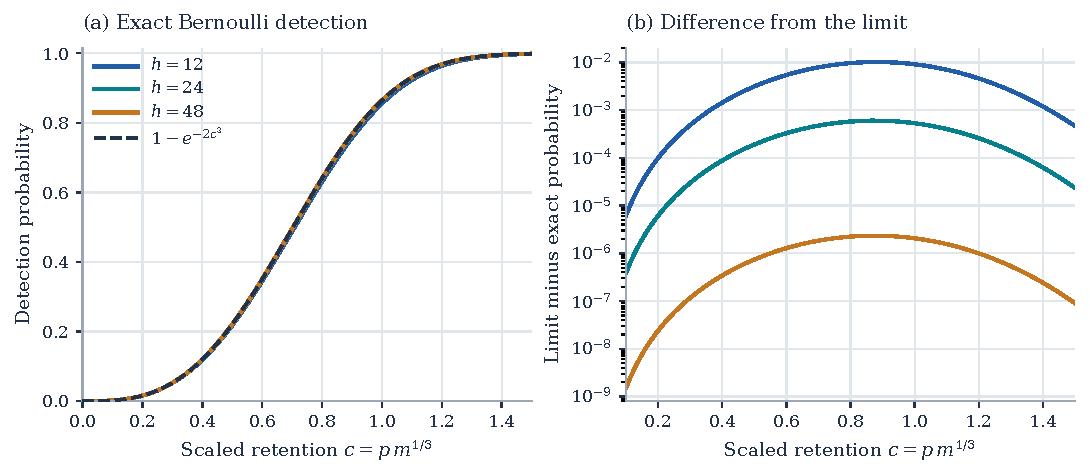
\includegraphics[width=\textwidth]{figures/balanced_sampling.pdf}
\caption{Exact Bernoulli detection probabilities from
\eqref{eq:bernoulli-exact}, with \(p=c m^{-1/3}\), compared with
\(1-e^{-2c^3}\). The right panel resolves the finite-depth deficit
on a logarithmic scale. The finite curves use independent retention;
\cref{thm:main-sampling} proves the same limiting law for fixed-size
uniform samples. The plot evaluates formulas and is not a simulation.}
\label{fig:balanced}
\end{figure}
